\chapter{Estado del arte}

Dada la naturaleza del producto, a lo largo del proyecto hablaremos largo y tendido sobre \textbf{dispositivos embebidos}, y por qué no, del \textbf{\textit{Internet de las Cosas}}, dado que pese a ser una máquina orientada al tratamiento del ejercicio físico requiere de conectividad, procesamiento de datos y transmisiones de información. Con el creciente ritmo al que progresa el ya famoso concepto \textit{``Internet de las Cosas''} (en inglés, \textit{IoT, Internet of Things}), se está apreciando un grandioso crecimiento en el desarrollo de los dispositivos y sistemas embebidos y/o de tiempo real.\\

De hecho, como dice \textit{Bruce Powel Douglass} hoy en día encontramos sistemas de este tipo que varían en tamaño y rendimiento, desde un reloj de muñeca inteligente hasta la automatización de los sistemas de control de una central nuclear \cite{real-time-uml-introduction}.\\

Por otro lado, según \textit{Matthew Evans}, el paradigma del \textit{IoT} nos permite ser más eficientes en tiempo y recursos a la hora de hacer las cosas \cite{whats-iot}. Se debe a que es más rápido implementar un sistema dedicado con unas necesidades muy claras a analizar y constituir un sistema completo de otro tipo. Esto deriva directamente en ahorro de producción y por tanto en unos márgenes de beneficio más flexibles para la empresa.\\

\section{Situación actual de la tecnología}

Como también dice \textit{Douglass}, hoy en día podemos encontrar sistemas dedicados y aplicaciones de tiempo real para todo propósito y en cualquier factor de forma. Por ejemplo, veamos algunos casos llamativos de hoy en día:\\

Un ejemplo de sistema empotrado podría ser el que encontramos en algunos negocios de comida rápida (en este caso, \textbf{\textit{McDonald's}}), que disponen de pantallas táctiles de gran tamaño permitiendo al usuario realizar su pedido a través de éstas, y posteriormente pasar por caja a recogerlo. Como sistema dedicado, se trata de un tipo de dispositivos con una utilidad muy específica y aislada, por lo que su implementación debe centrarse siempre en la máxima representación de ésta.

\begin{figure}[H]
	\centering
	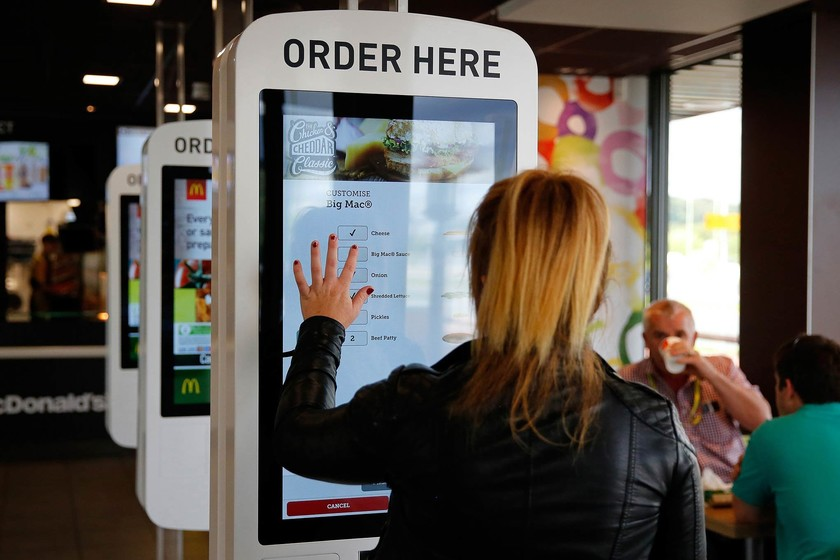
\includegraphics[width=0.75\linewidth]{imagenes/pedido-pantalla-tactil.jpg}
	\caption{Pantallas táctiles para realizar pedidos en McDonald's - Fuente: \textit{Mientras Tanto En México} \cite{mcdonalds-pantalla-tactil-pedidos}}
\end{figure}

Por otra parte, nos encontramos con la empresa alemana \textbf{\textit{gridX}} \cite{gridx}. Se trata de una empresa proveedora de energía limpia en Alemania que, además de apostar por las energías renovables y su administración de forma transparente, comercializan el dispositivo \textbf{gridBox}. Se trata de un sistema embebido que actúa a modo de contador y administrador inteligente con todo el consumo de dicha energía, optimizando el uso de ésta en el hogar.

\begin{figure}[H]
	\centering
	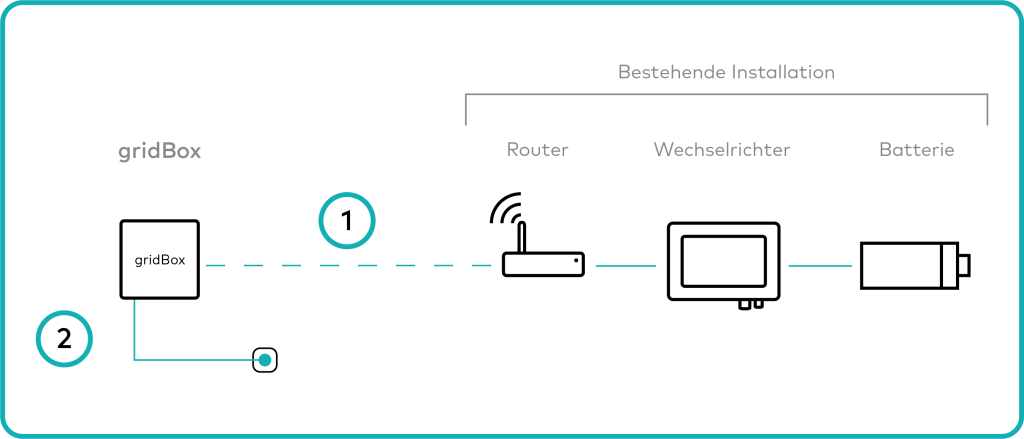
\includegraphics[width=0.75\linewidth]{imagenes/gridbox-utility.png}
	\caption{Instalación de gridBox en el hogar. De una toma de corriente a todos los dispositivos, pasando por el router - Fuente: \textit{Web oficial de gridX} \cite{gridbox}}
	\label{gridbox-installation}
\end{figure}

Además de ser un sistema dedicado con este propósito tan específico, implementa conexión de red para poder monitorizar los datos y transferirlos a aplicaciones de móvil y/o escritorio a los dueños de la casa. Y por último, el producto lleva integrado un sistema de actualizaciones \textit{OTA} con \textit{Mender.io}, herramienta de la que hablaremos extensamente más adelante.\\

A modo de último ejemplo, nos encontramos con \textbf{\textit{Kinestral}} \cite{kinestral}; una compañía con sedes en Norteamérica y Taiwan que focaliza su negocio en \textit{la transformación del cristal}. Comercializan el producto \textbf{\textit{Halio}}, que se trata de una especie de vidrio inteligente para cualquier propósito (sobre todo, el de la instalación en edificios) que posee la particularidad de \textbf{oscurecerse automática o manualmente} para sombrear y reducir el impacto de los deslumbramientos de la luz solar.

\begin{figure}[H]
	\centering
	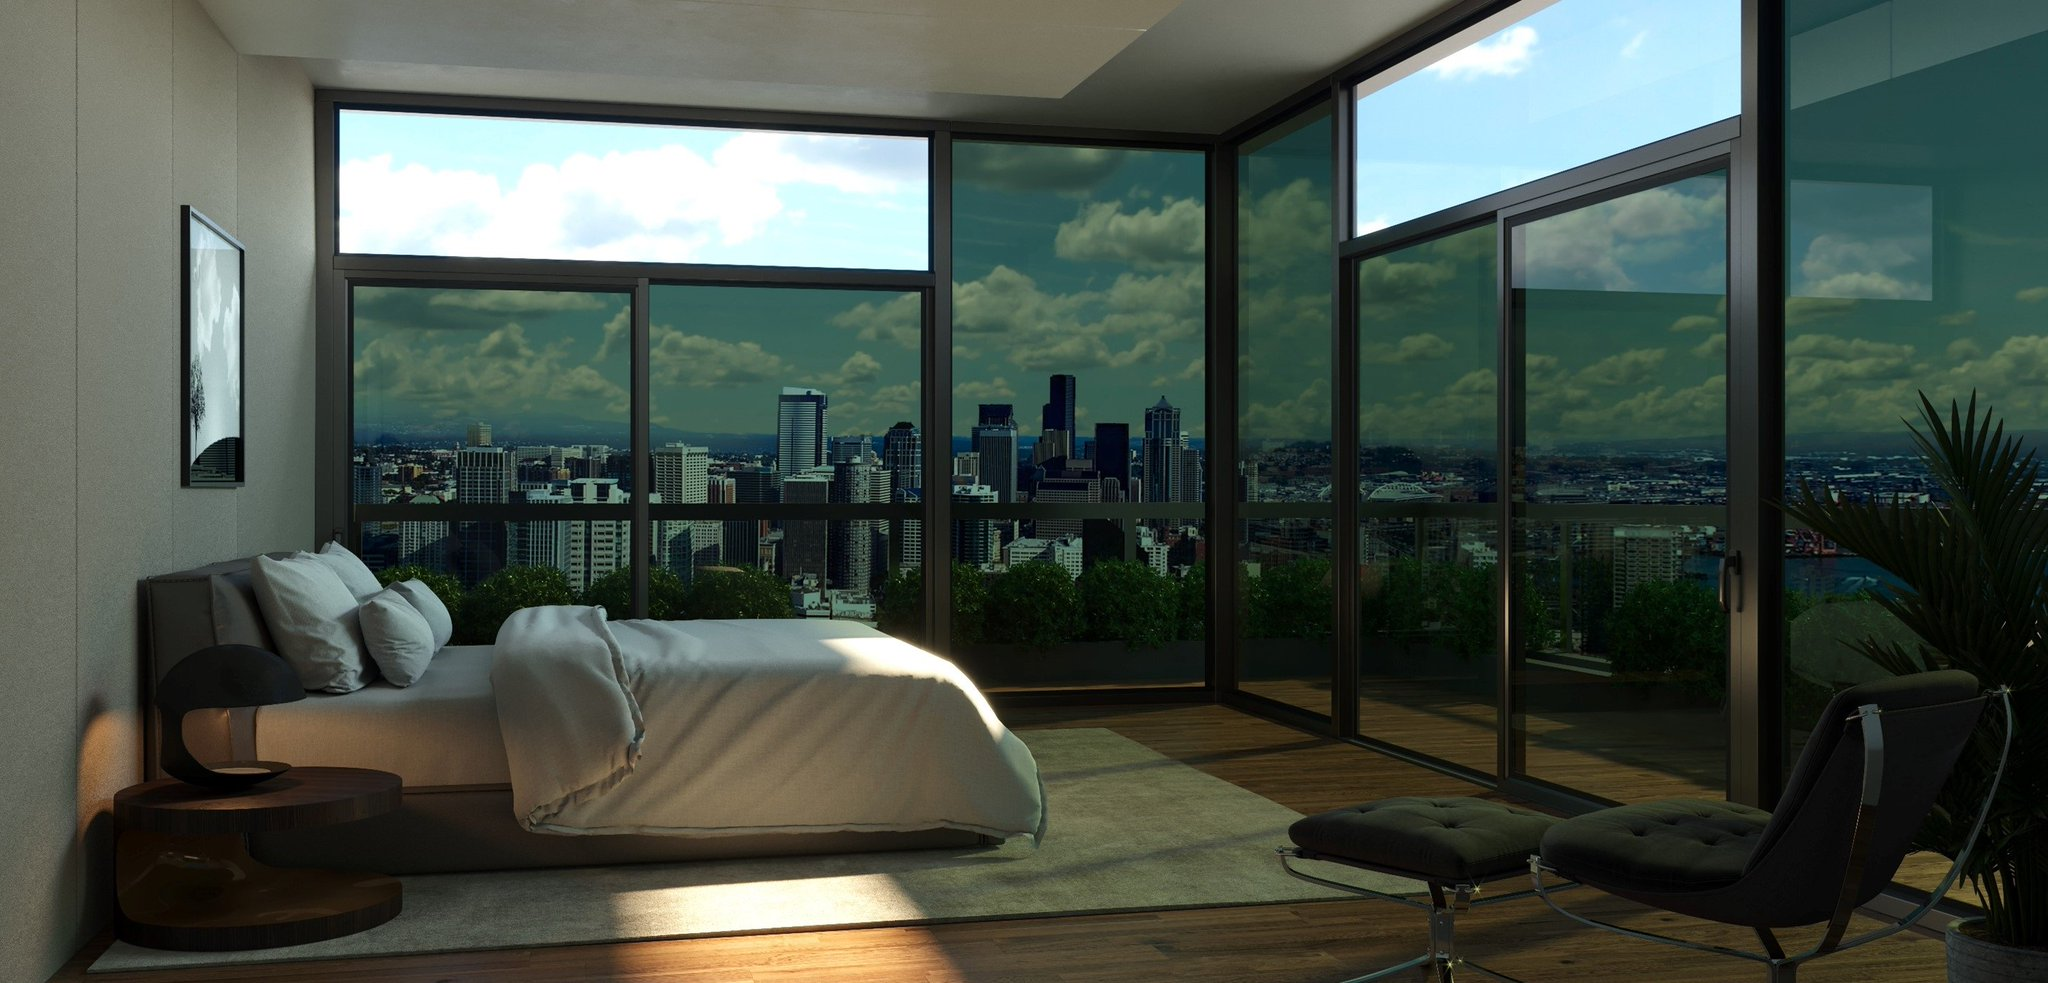
\includegraphics[width=0.8\linewidth]{imagenes/halio-glass.jpeg}
	\caption{Ejemplo de instalación de Halio Glass en el hogar - Fuente: \textit{Cuenta de Twitter oficial de Halio Glass (producto de Kinestral)} \cite{halio-glass}}
	\label{halio-glass}
\end{figure}

Además de esta funcionalidad tan curiosa e innovadora, incorporan la conexión con una aplicación móvil desde la que poder controlar de manera independiente cada uno de los paneles instalados en el edificio. Por último, también incorporan un sistema de actualización basado en \textit{Mender.io}.\\

\noindent\makebox[\linewidth]{\rule{\textwidth}{0.4pt}}\\

Una vez vistas algunas implementaciones de la tecnología, dado el propósito del proyecto en este apartado tenemos que distinguir entre dos grandes campos, \textbf{sistemas operativos embebidos} y \textbf{métodos de actualización}.\\

Antes de hablar de sistemas operativos empotrados, debemos concretar la idea de ``dispositivo embebido'' (o \textit{dedicado}) como tal. Para \textit{Jean Paul Calvez}, consiste en lo siguiente:

\begin{quotation}
	``Un sistema dedicado quiere decir que éste es desarrollado para satisfacer una necesidad muy concreta en un momento dado. Su límite de operatividad está definido en varios años o décadas, por lo que la durabilidad es importante. El sistema debería ser \textit{lo más perfecto posible}, siendo lanzado en su versión final con tecnologías actuales. Sus posibilidades de futuro desarrollo están limitadas a unas pocas mejoras para la misma aplicación. Por lo tanto, ni se trata de un ordenador de propósito general ni de un prototipo que funciona bien solo en un momento concreto. [...] La técnica implementada ha de ser correcta y adecuada para reducir costes y tiempo de desarrollo.'' - \textit{Jean Paul Calvez} \cite{embedded-real-time-systems-embedded-systems}
\end{quotation}

Entre las técnicas de implementación se encuentran el uso de sistemas completos (como microcomputadores, terminales o sistemas de procesamiento de imágenes) en contraposición al uso conjunto de placas de desarrollo, fuentes de alimentación y placas con microprocesador entre otras herramientas.\\

En cuanto a hardware suele darse el caso de \textbf{la reutilización}, no ya en el software; dado que en el primer caso es mucho mayor el coste de la creación de nuevos componentes, por lo que se prefiere reutilizar cosas que ya existen.\\

\noindent\makebox[\linewidth]{\rule{\textwidth}{0.4pt}}\\

Por una parte, los dispositivos embebidos están teniendo un gran crecimiento dadas las mejoras computacionales de rendimiento y consumo, permitiendo desarrollar sistemas aislados que desempeñan funciones muy específicas, como recopilar datos y transmitirlos (como una granja de dispositivos que implementan el protocolo \textit{ZigBee} \cite{zigbee-products}), o actuar de entorno multimedia para diversos fines (como los sistemas de navegación automovilísticos inteligentes, a menudo programados utilizando \textit{Qt Automotive Suite} \cite{qt-automotive}).\\

Principalmente, estos productos se desarrollan a partir de un \textbf{ordenador de placa reducida} (en inglés: \textit{Single Board Computer}, o \textit{SBC}); como lo son la \textit{Raspberry Pi} \cite{raspberry-pi}, la \textit{Tinker Board} de \textit{ASUS} \cite{asus-tinkerboard} o \textit{Arduino} en sus diferentes versiones \cite{arduino-store}. O bien, el equipo encargado de desarrollar el producto puede optar por diseñar una placa a medida que satisfaga las necesidades del proyecto. Para ésto, es necesaria una gran estimación de las ventajas con respecto al precio, y un desarrollo de software muy estrechamente ligado al del hardware.\\

Ahora bien, sobre estas plataformas hardware se pueden utilizar diferentes sistemas operativos, dando prioridad a la elaboración de uno propio a partir de diversas herramientas (como \textit{OpenEmbedded/Yocto Project} \cite{yocto-project}, \textit{Buildroot} \cite{buildroot} o \textit{Linux from scratch} \cite{linux-from-scratch}); ya que aseguran una mayor modularidad y ligereza en cuanto a dependencias (no se instala nada que no sea necesario). Estas tecnologías suelen ser de código abierto, libres y gratuitas, aunque existen alternativas diferentes más específicas para este tipo de desarrollos. Por ejemplo, existe \textbf{\textit{Qt for Device Creation} (Qt para creación de dispositivos embebidos)}, que se basa en el \textit{Proyecto Yocto} incorporando las dependencias necesarias para lanzar de forma automática una aplicación embebida desarrollada con el conocido marco de trabajo Qt.

\begin{quotation}
	``En cuanto a Linux embebido, \textit{Qt for Device Creation} provee del stack \textit{Boot to Qt} (inicia a Qt). Es un stack de software ligero y optimizado con Qt para sistemas Linux embebidos que es instalado directamente en el dispositivo de destino. Provee de una serie de herramientas requeridas para un desarrollo más rápido y un menor tiempo de puesta en el mercado'' - \textit{Qt Documentation} \cite{qt-device-creation}
\end{quotation}

Se trata de una alternativa comercial interesante para empresas dedicadas a este tipo de desarrollos, aunque no es nada asequible para estudiantes o programadores que no deseen una licencia comercial, ni para empresas pequeñas o \textit{start-ups} dado que el coste es muy elevado.\\

\noindent\makebox[\linewidth]{\rule{\textwidth}{0.4pt}}\\

Por otro lado, encontramos \textbf{el sistema de actualizaciones}. En estos últimos años durante los que el \textit{IoT} ha ido tomando una popularidad progresiva, es cada vez más importante hablar de protección y seguridad. Por ejemplo, en 2017 un grupo chino hackeó el sistema de un coche inteligente \textit{Tesla} por segunda vez, manejando el sistema dedicado a su antojo \cite{tesla-system-hacked}.\\

Para evitar manipulaciones como ésta o denegaciones de servicio que podrían dejar bloqueados los dispositivos, es imprescindible una seguridad \textit{óptima}; además de un sistema de actualizaciones que permita al dispositivo recuperarse de los errores.\\

[TO DO]

\subsection{Contexto actual en cuanto a modelos de desarollo}

Como señala \textit{Bruce Powel Douglass} en el apartado 1.3 de su libro \textit{Real-time UML. Developing efficient objects for embedded systems} \cite{real-time-uml-model-based-development}, el proceso de desarrollo de software actual debe cimentarse sobre varios principios importantes:

\begin{itemize}
	\item Desarrollo iterativo: se debe centrar la atención en exponer los riesgos y mitigarlos. Para un software efectivo, el desarrollo ha de dividirse en piezas y/o prototipos rápidos de calidad.
	\item Desarrollo basado en modelos: un sistema complejo no puede ser ensamblado usando solo construcciones a nivel de código. Los modelos abstractos permiten capturar las características importantes de la aplicación y la forma en que se relacionan independientemente de la implementación a bajo nivel.
	\item Asociación bidireccional entre \textbf{código} y \textbf{modelo}: el código y los diagramas deben ser diferentes vistas del mismo modelo intrínseco. Si el código se desvía del modelo diseñado, el mantenimiento por separado se vuelve pesado y el sistema pasa a sostenerse solo por el código; lo que lo convierte en más difícil de mantener.
	\item Modelos ejecutables: solo se pueden probar cosas que se ejecutan, por lo que hay que ejecutar pruebas \textbf{pronto} y \textbf{a menudo}. La clave es transformar el diseño en algo que puede ser ejecutado en el orden de segundos o minutos, en lugar de las aproximaciones tradicionales manuales que tardan semanas y/o meses.
	\item Abstracción en el nivel de diseño: dadas las aplicaciones complejas de hoy en día, usamos modelos abstractos para ayudarnos a entender e implementarlos. Debemos testearlos al mismo nivel.
	\item ``Prueba lo que despliegas y despliega lo que pruebas'': el propósito de testear modelos ejecutables permite desarrollar aplicaciones sin defectos de forma rápida (usando las tecnologías apropiadas) para un desarrollo iterativo veloz donde los tests \textit{solo necesitan hacerse una vez}.
\end{itemize}

Douglass propone el uso del lenguaje \textit{UML (Unified Modelling Language, o Lenguaje de Modelado Unificado)} para alcanzar estos fines, siguiendo una metodología desarrollada por él mismo llamada \texttt{ROPES} (\textit{Rapid Object-Oriented Process for Embedded Systems}, en español: ``Proceso rápido orientado a objetos para dispositivos embebidos''). Se trata de un paradigma interesante para llevar a la práctica en equipos de desarrollo en los que las tareas de implementación del hardware y el software se separan para luego unirse. Sin embargo, en este proyecto estaremos hablando de la infraestructura virtual que soporta al software, no ya sobre las aplicaciones embebidas como tal.

\section{Problemas que se desean resolver}

La solución planteada por este proyecto tiene que ver con la necesidad de un sistema operativo embebido para un uso específico, en contraposición a sistemas ya existentes que incorporan paquetes innecesarios para este fin o permiten una mucho menor customización (como lo son \textit{Raspbian} \cite{raspbian}, \textit{Windows 10 IoT} \cite{windows-10-iot} o \textit{Ubuntu Mate} \cite{ubuntu-mate-raspberry} entre otros). Esto permitirá sufrir un \textbf{menor tiempo de arranque} además de disponer de \textbf{detalles estéticos} (como la no inclusión de mensajes del kernel durante su carga y la muestra de una imagen a lo largo del proceso). Todas las decisiones tomadas para este fin se habrán hecho pensando en la mayor conveniencia para el proyecto DYNAsystem.\\

Por otro lado, el sistema de actualizaciones juega \textbf{un papel muy importante} en este proyecto, dado que intenta romper con el paradigma de actualizaciones \textit{OTA} a través de conexión a Internet cableada, permitiendo desplegar nuevas versiones del software \textbf{de forma inalámbrica y segura} a través de un servidor centralizado. Para ello, se habrán valorado los diferentes servicios de actualización y se habrá tomado una decisión de inclusión en el proyecto.

\newpage
